\documentclass[]{article}
\usepackage[german]{babel}
\usepackage{graphicx}
\usepackage{tabularx}
\usepackage[backend=bibtex, natbib=true]{biblatex}
\usepackage{listings}
\usepackage{tikz}

\lstset{%
	basicstyle=\ttfamily\scriptsize,        % Code font, Examples: \footnotesize, \ttfamily
	keywordstyle=\color{blue!80!black},     % Keywords font ('*' = uppercase)
	commentstyle=\color{gray},              % Comments font
	numbers=left,                           % Line nums position
	numberstyle=\tiny,                      % Line-numbers fonts
	stepnumber=1,                           % Step between two line-numbers
	numbersep=5pt,                          % How far are line-numbers from code
	backgroundcolor=\color{gray!10!white},  % Choose background color
	frame=none,                             % A frame around the code
	tabsize=2,                              % Default tab size
	captionpos=b,                           % Caption-position = bottom
	breaklines=true,                        % Automatic line breaking?
	breakatwhitespace=false,                % Automatic breaks only at whitespace?
	showspaces=false,                       % Dont make spaces visible
	showstringspaces=false                  %
	showtabs=false,                         % Dont make tabls visible
	columns=flexible,                       % Column format
	morekeywords={},                        % Specific keywords
	stringstyle=\color{green!50!black},%
}%

\bibliography{bibliography}
%opening
%Here you can enter your names and titleof your report
\title{Dokumentation - Luftqualität in Innenräumen - Gruppe 1}
\author{Friedrich Just 1326699 \\ Stipe Knez 1269206 \\ Lucas Merkert 1326709 \\ Achim Glaesmann 1309221 \\ Max-Rene Konieczka 1211092 \\ Can Cihan Nazlier 1179244}

\begin{document}

	\begin{titlepage}
		\maketitle
		\thispagestyle{empty}
	\end{titlepage}
	\tableofcontents
	\setcounter{page}{1}
	\newpage
	
	
	\section{Projektthema}
	Die durch Covid-19 verursachte Pandemie prägte die letzten 2 Jahre fast der gesamten Welt. Insgesamt forderte die Krankheit etwa 5,18 Millionen Menschenleben. Dennoch ist das Thema aktueller denn je. Europaweit steigen die Infektionszahlen auf nie dagewesene Werte, während die im Sommer verabreichten Impfungen langsam an Effektivität verlieren. Ein Hauptrisiko zur Infektion besteht dabei in Innenräumen. Unser Auftrag besteht nun darin, ein System zu entwickeln welches in der Lage ist, das Infektionsrisiko einzelner Räume eines Gebäudes einzuschätzen und so einen Richtwert für den Anwender darstellt, wie er sein Verhalten diesem Wert anpassen kann. Realisiert werden soll dieses System über die Verwendung verschiedener Sensoren zur Erfassung mit dem Infektionsrisiko direkt verknüpfter physikalischer Größen. Die zur Ansteckung, vermutlich, wichtigen Aerosole, können dabei nur bedingt durch Masken zurückgehalten werden, es macht also Sinn abzuschätzen inwieweit die Luft eines Raumes durch Aerosole belastet ist. Da die direkte Messung von Aerosolen zeitaufwendig und schwer umsetzbar ist, konzentrieren wir uns hierbei auf Werte, die einen direkten Rückschluss auf die Ausatemmenge der Personen im Raum ermöglichen. Mit der Annahme, dass die Aerosolkonzentration dabei direkt abhängig zur Ausatemmenge ist.\newline
	Um dies zu erreichen, bedienen wir uns folgender Sensoren: Dem CCS811 von Adafruit, dem SCD41 und dem SHT21 von Sensirion. Der CCS881 ist ein energieeffizienter digitaler Gassensor, welcher über die Verwendung eines Metalloxidsensors ein breites Spektrum an flüchtigen organischen Verbindungen messen kann. Diese gibt der Sensor als CO2-Äquivalente an. Der CO2-Äquivalenzbereich geht hierbei von 400ppm bis 8192ppm. Eine Kompensation für Abweichungen durch Temperatur und Luftfeuchtigkeit ist dabei über einen externen Feuchtigkeits- und Temperatursensor möglich. Dies ermöglicht in Verbindung mit einem Mikrokontroller die Überwachung der Luftqualität. Der Sensor enthält dabei eine I²C-Schnittstelle sowie einen Analog-Digital-Converter.
	Der SHT21 ermöglicht die Messung der relativen Luftfeuchtigkeit so wie der Temperatur mit einer Genauigkeit von ±2\% relativer Luftfeuchtigkeit so wie ±0.3° Celsius bezüglich der Temperatur.\newline
	Beim SCD41 Sensor handelt es sich um einen miniaturisierten CO2-Sensor basierend auf dem photoakustischem Sensorprinzip. Dabei wird über einen im Sensor integrierten SHT41 Feuchtigkeits- und Temperatursensor eine chipinterne Signalkompensierung ermöglicht. Die Genauigkeit des SCD41 beträgt dabei im Bereich von 400 ppm – 5’000 ppm ± (40 ppm + 5\% des abgelesenen Wertes). Beide Sensoren von Sensirion können über die I²C-Schnittstelle angesprochen werden. Genauere Informationen zu den Sensoren sind im Unterkapitel Sensoren vermerkt.\newline
	Die so ermittelten Daten sollen anschließend in eine graphische Darstellung in Form einer Ampelindikation überführt werden, um dem Anwender eine direkte Bewertung der Gefahrenlage zu ermöglichen. Die Kommunikation zwischen Mikrocontroller und Sensoren soll dabei via I²C-Schnittstelle erfolgen, die Kommunikation zwischen den einzelnen Mikrokontrollern auf Basis des ZigBee-Protokolls. Um dies zu ermöglichen wurde entschieden, einen Microcontroller auf Basis des Atmega256rfr2-Chips zu verwenden, welcher die Verwendung beider Übertragungsprotokolle ermöglicht, so wie eine serielle Kommunikation über eine UART-Bridge. Die ermittelten Daten werden wie erwähnt seriell an eine von uns entwickelte Applikation auf einem leistungsfähigeren Endgerät übermittelt, welches die Daten auswertet und in ein graphisches Modell des zu beschreibenden Zimmers einbettet. Das Frontend der Applikation soll dabei mittels JavaScript realisiert werden, während das Backend in Java zu verwirklichen ist. Die Applikation soll es dem Anwender grundsätzlich ermöglichen eigene Grundrisse zu zeichnen, Räume zu definieren und Sensoren in diesen zu platzieren. Die ermittelten Werte der Sensoren sollen dabei einmal innerhalb von Graphen zeitlich dargestellt werden sowie die über einen eigens zu entwickelnden Algorithmus errechnete Gefahrenlage mittels eines Ampelsystems einmal innerhalb der Anwendung als auch über eine am jeweiligen Funkmodul angebrachte LED dargestellt werden. 
	
	\section{Aufgabenaufteilung} %kurze aufgabenteilung
	Zu Beginn des Projektes wurde entschieden die Aufgaben in zwei Teile aufzuteilen, einerseits in einen Sensorteil und andererseits in einen Applikationsteil. Es wurde festgelegt, dass Herr Merkert, Herr Just und Herr Glaesmann für die Einrichtung und Programmierung der Sensoren zuständig sind, während Herr Knez, Herr Nazlier und Herr Konieczka für die Einrichtung eines Servers und die Entwicklung der Applikation zuständig sind. 
		\subsection{Friedrich Just}
		\subsection{Stipe Knez}
		\subsection{Lucas Merkert}
			Aufgabe von Herr Merkert war die Programmierung des CCS811 Sensors sowie verschiedene administrative Aufgaben.
		\subsection{Achim Glaesmann}
		\subsection{Max-Rene Konieczka}
		\subsection{Can Cihan Nazlier}
		
	\section{Ergebnisse der Recherche}%Lucas/Achim Friedrich
	\section{Lösungsansatz} %detaillierte beschreibung der einzelnen Aufgaben, probleme und Lösungen
		%TODO different subsections wer was wie gelöst hat und welche Probleme aufgetreten sind, dabei angeben welche Standards/werkzeuge/equipment genutzt worden sind
		\subsection{SHT21}
		\subsection{SCD41}
		\subsection{CCS811}
			Der CCS811 \cite{ccs_datasheet}ist ein Sensor von ams, der den äquivalenten CO2 (eCO2) Gehalt und den Gehalt der totalen flüchtigen organischen Verbindungen (TVOC) in der Luft messen kann. Dabei kann eCO2 von 400ppm bis 8192ppm, TVOC von 0ppb bis 1187ppb gemessen werden und ein Messintervall von 250ms, 1s, 10s, 60s festgelegt werden. Die Pin-Beschreibungen kann man in Abbildung \ref{img:ccs_pintable} sehen. Wichtig sind hiervon die Pins:
			\begin{itemize}
				\item VDD: Anschluss an 3,3V als Versorgungsspannung (min 1,8V)
				\item nWAKE: Anschluss an GND (active low), damit der Sensor durchgehend aktiv ist
				\item SDA: Data Anschluss für I2C, wird mit einem SDA Pin des Zigbee-Boards verbunden
				\item SCL: Clock Anschluss für I2C, wird mit einem SCL Pin des Zigbee-Boards verbunden
				\item GND: Ist nicht in der Tabelle angegeben, muss aber mit GND auf dem Zigbee-Board verbunden werden
			\end{itemize}
			\begin{figure}[!h]
				\centering
				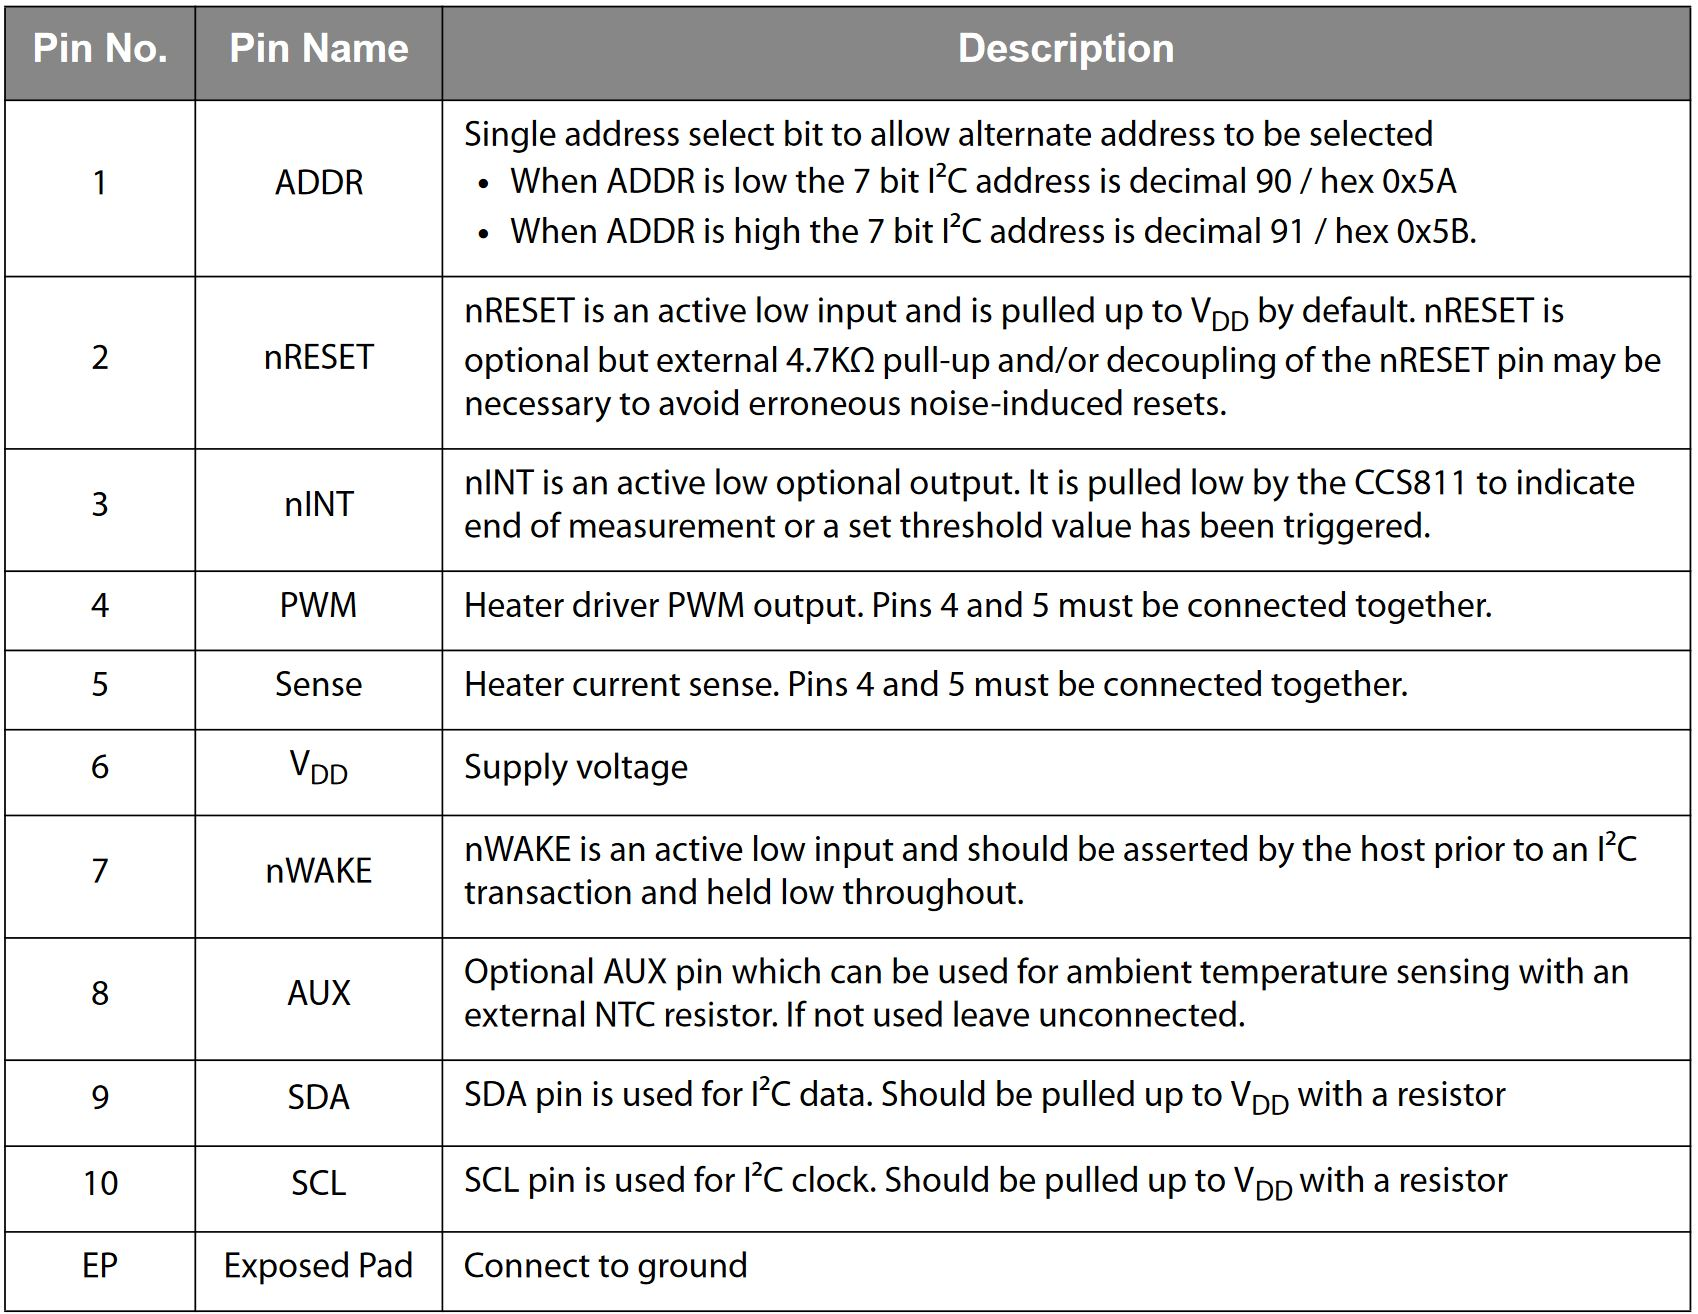
\includegraphics[scale=0.50]{images/ccs_pintable}
				\caption{Tabelle mit den Beschreibungen der Pins des CCS811}
				\label{img:ccs_pintable}
			\end{figure}
			In Abbildung \ref{label} ist das Zustandsdiagramm des CCS811 Sensors dargestellt. Zustände die nicht mit dem Sensor interagieren sind hier nicht dargestellt. Zu Beginn wird 2000 ms gewartet da der SCD41 Sensor entsprechende Zeit zum starten braucht. Die eigentliche Startzeit des CCS811 beträgt maximal nur 20ms. Der Zugriff auf den Sensor über den I2C-Bus spricht die Adresse 0x5A an, da der ADDR Pin nicht gesetzt ist. Im APP\_RESET\_CSS\_SW\_STATE wird mit 0xFF das SOFTWARE\_RESET\_REG angesprochen und der Befehl 0x11 0xE5 0x72 0x8A geschrieben. Dieser Befehl dient dazu einen versehentlichen Software Reset zu verhindern. Ist diese Sequenz geschrieben worden, befindet sich der Sensor im Boot mode. Zwischen den einzelnen I2C-Befehlen wird immer 1ms gewartet um sicherzugehen, das der Befehl richtig ausgeführt werden kann. Dies führt zwar zu einem erhöhten Zeitaufwand, ist jedoch unbedenklich, da der Messintervall 60 s beträgt und somit genügend Zeit zur Verfügung steht. Im nächsten Schritt wird das HW\_ID\_REG angesprochen und im darauf im folgenden Zustand auch ausgelesen. Hierbei ist wichtig, dass die HW\_ID 0x81 ist. Im APP\_CCS\_CHANGE\_TO\_APPSTATE\_STATE wird mit dem Befehl 0xF4 zurück in den Appstate gewechselt. Nun wird das MEAS\_MODE\_REG 0x01 angesprochen und der Befehl 0x30 geschrieben. Dieser Befehl setzt den Messintervall auf 60s, welcher den geringsten Stromverbrauch hat. Zum Testen der Applikation wurde hier ein kürzerer Intervall gewählt. Zudem werden keine Interrupts gesetzt die feuern würden wenn Daten vorhanden wären. Um zu überprüfen ob die Messung funktioniert, wird nun 60s gewartet und dann das STATUS\_REG 0x00 überprüft, ob Daten vorhanden sind. Ist dies der Fall, ist das 3. Bit gesetzt. Falls ein Fehler auf dem I2C-Bus oder dem Sensor aufgetreten ist, könnte man dies über das 0. Bit feststellen und im Register 0xE0 auslesen. Sind Daten zum abrufen bereit, werden die Sensoren SHT21 und SCD41 initialisiert. Dabei wird auch der Messtimer von 60s gestartet. Sind diese 60s abgelaufen, so wird das ALG\_RESULT\_DATA\_REG 0x02 angesprochen in dem die bereits berechneten Daten der Messung bereit liegen. Diese werden als 4 Byte ausgelesen, wobei die Bytes 0 und 1 den eCO2 Wert beinhalten und Byte 3 und 4 den TVOC Wert.
			\begin{figure}[!h]
				\centering
				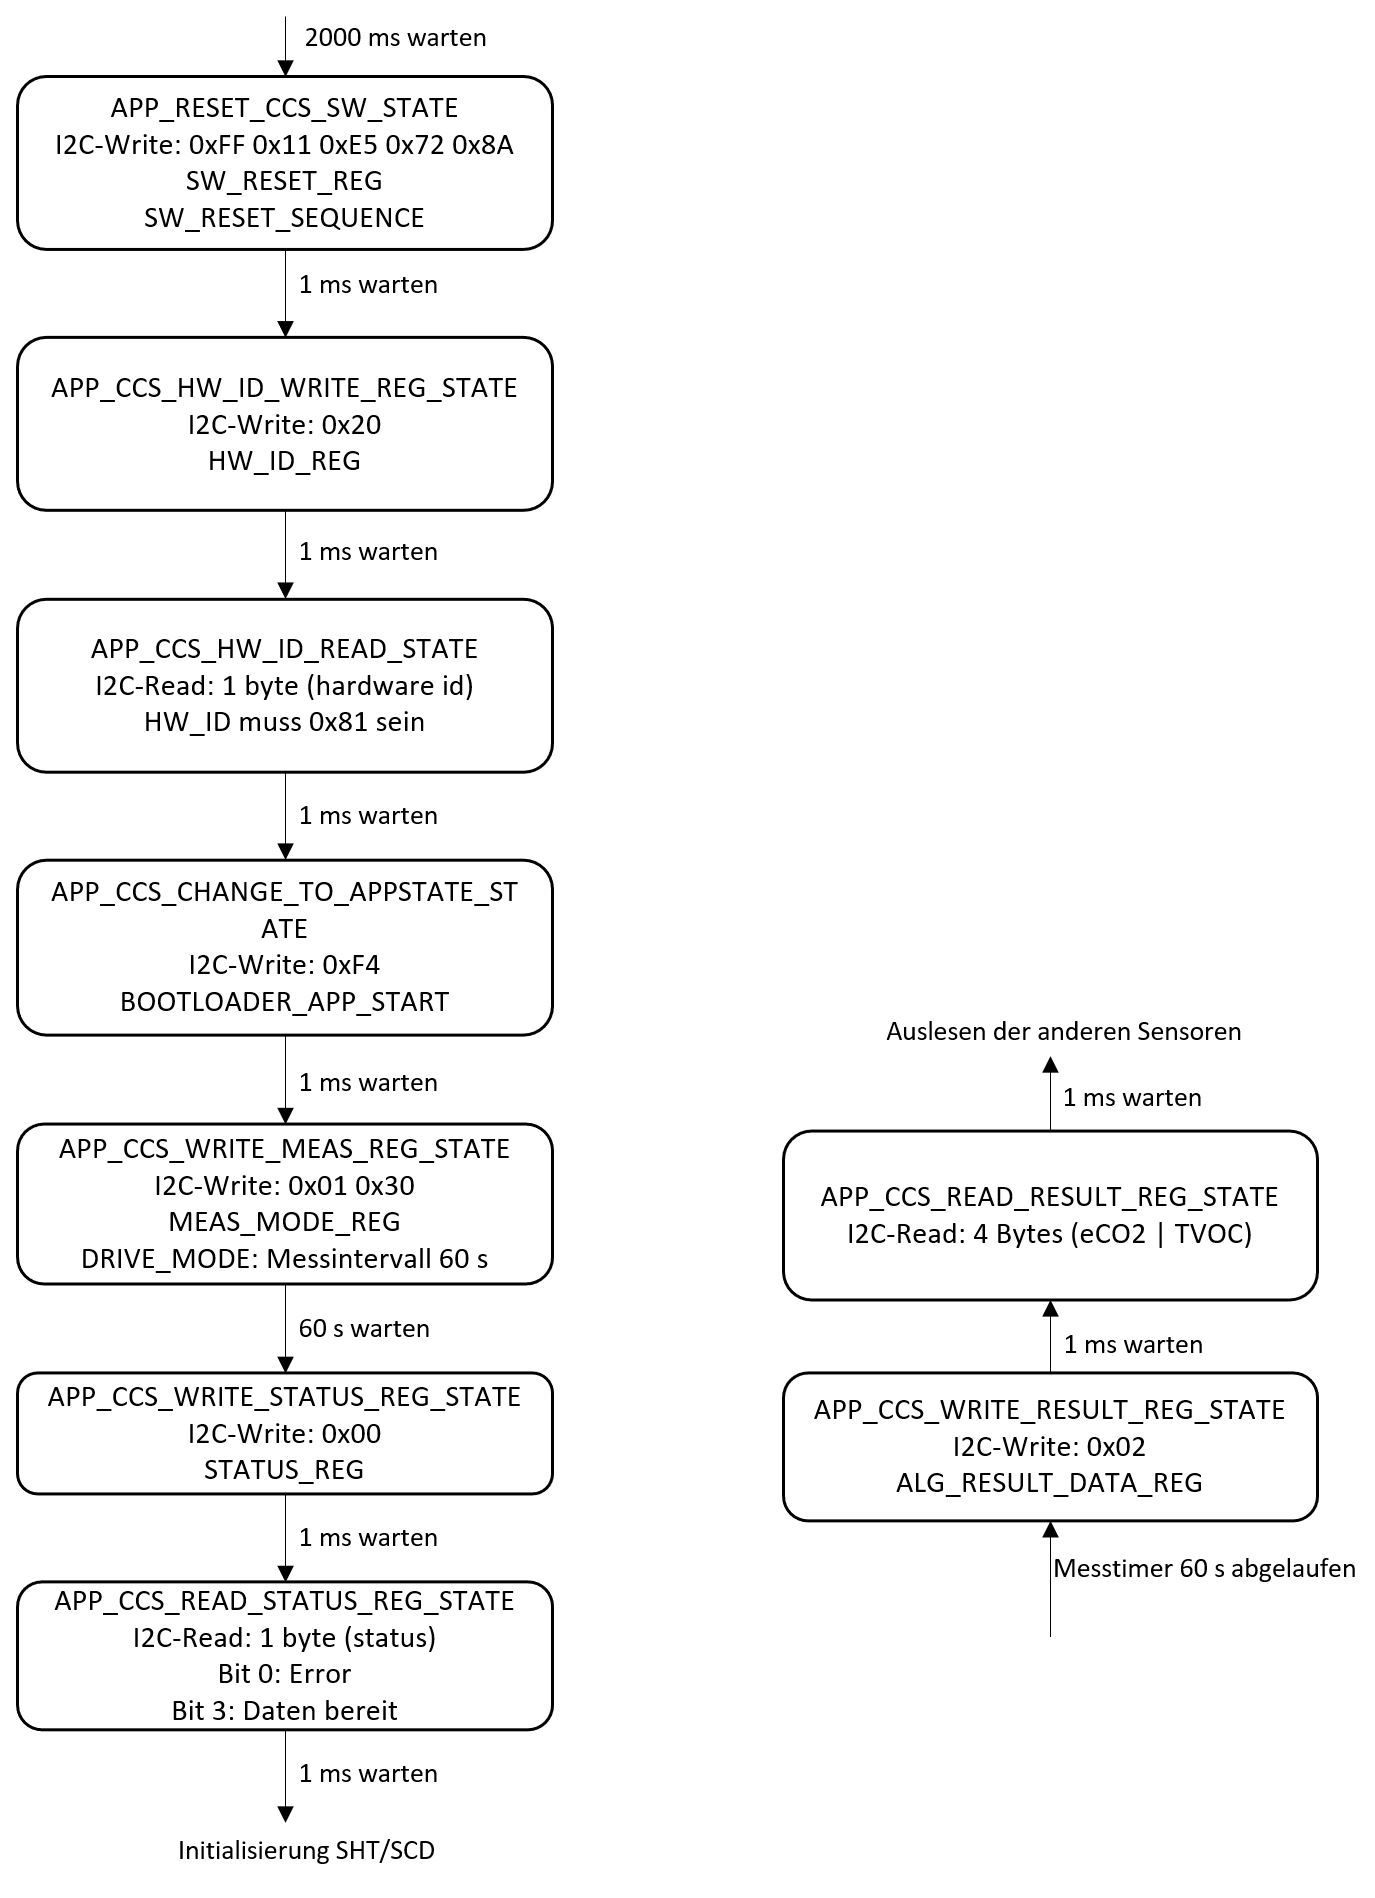
\includegraphics[scale=0.30]{images/ccs_zustandsdiagramm}
				\caption{Zustandsdiagramm des CCS811 Sensors, rechts: Initialisierung, links: Auslesen der Werte}
				\label{img:ccs_zustandsdiagramm}
			\end{figure}
			\subsection{Probleme bei der Programmierung des CCS811}
				Da sich der CCS811 in seiner Funktionsweise von den anderen beiden Sensoren unterscheidet, war es zu Anfang schwierig einen richtigen Ansatz zu bekommen. Vor allem das Wechseln in den Bootmodus war erst nach der Erläuterung in der Vorlesung klar und damit auch nachvollziehbarer. Zudem haben teilweise die Funkmodule nicht richtig Funktioniert, da entweder überhaupt nichts über die UART ausgegeben werden konnte oder die bei einem I2C-Befehl der Callback mit Error zurück gekommen ist. Nachdem wir den Code mehrmals auf Richtigkeit der Befehle und Ablauf überprüft haben, haben wir das ZigBee-Board ausgewechselt und das Messen hat ohne Probleme funktioniert. Was dabei der genaue Fehler war ist uns nicht bekannt. Zudem war die Funktion der Pins nWAKE und ADDR zu Anfang nicht klar. Der nWAKE Pin ist dafür da damit der Sensor aktiv ist und muss dafür auf low gezogen werden. Also haben wir diesen and GND angeschlossen und somit ist der Sensor durchgehend aktiv. Der ADDR Pin gibt an ob die I2C-Adresse des Sensors 0x5A oder 0x5B ist. Da der ADDR Pin nicht angeschlossen ist, ist die I2C-Adresse 0x5A.
				%TODO funktionsweise eines Metall  oxid Sensors, entweder hier oder in REcherche
	\section{Ausblick und Erweiterungsmöglichkeiten}
		
		

%----------------------------------------------------------------------------
% Bibliography
%----------------------------------------------------------------------------	
\printbibliography
\end{document}
